\chapter{An\'alisis del sistema}
\section{Identificaci\'on de problemas y oportunidades b\'asicas}
En el estudio del sistema, se encontraron los siguientes problemas:%
\\
\begin{itemize}
\item El sistema debe ser flexible y parametrizable.%
\item El volumen del flujo de datos es muy grande.%
\item El registro de las ventas puede llegar a no estar acorde a la realidad.%
\item Los participantes pueden llegar a perder la tarjeta en la que se les realiza la consignaci\'on.%
\end{itemize}%
%
\begin{figure}[htbp]
%centering es para centrar la imagen
	\centering
%aca es donde se incluye la imagen, se da el ancho(width), \textwidth significa que con repescto al tamano del
%texto y luego la ruta, relativa siempre es decir, a partir de donde se esta, como images esta ahi
%dentro, solo se usa desde images y ojala nada de espacios en el nombre de la imagen
		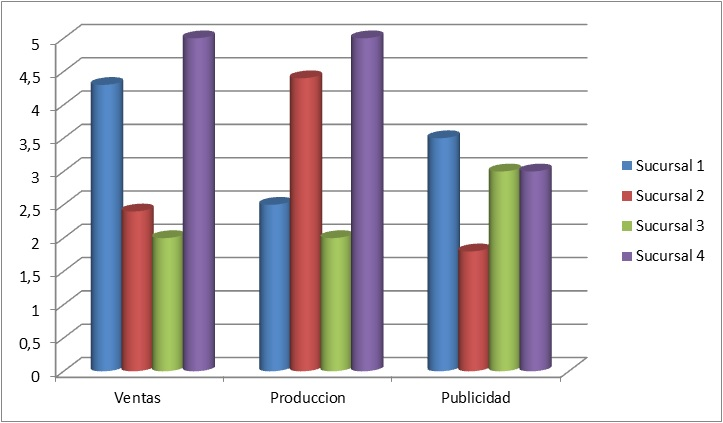
\includegraphics[width=0.60\textwidth]{images/Eficienciadelasucursal.jpg}
%el caption es para el texto que aparece debajo de la imagen
	\caption{Eficiencias de las sucursales}
%label es para darle una referencia, por ejemplo si uno dice "como se puede ver en la imagen a1"
	\label{fig:eficienciasucursales}
\end{figure}%
%
\section{Evaluaci\'on del beneficio del proyecto}
Lo beneficios de el sistema de informaci\'on que se va a implementar nos permitir\'a consultar, observar y verificar la informaci\'on de la compa\~n\'ia en tiempo real y efectiva, de tal forma que estos procesos puedan ser flexibles y f\'acil de manejar para el usuario, esto nos lleva a que se Incrementara  el entendimiento del uso de las Tecnolog\'ias de Informaci\'on en la organizaci\'on y posteriormente  incrementar las ventas; para llevar esto a cabo, es necesario ser el primero en proporcionar informaci\'on a clientes potenciales sobre un producto en particular. y mantener una relaci\'on con ellos a trav\'es de informaci\'on permanente.%
%
\subsection{?`Vale la pena trabajar en este proyecto?}
Hoy en d\'ia se esta tomando conciencia de la importancia dentro de las organizaciones de manejar los ambientes de negocio implementando un sistema de informaci\'on, lo fundamental para una compa\~n\'ia es un mercado globalizado a nivel competitivo, que tanto la estrategia de negocios y estrategias tecnol\'ogicas est\'en bajo un mismo esquema.%
\\%
\\%
Por lo anterior vale la pena trabajar en este proyecto ya que se ve reflejado la fusi\'on de estas dos estrategias, por una parte se esta trabajando los procesos del negocio y por el otro, se menejara un sistema que ayudar\'a a que todos estos procesos se realicen en forma automatizada, con el fin de alcanzar las metas y objetivos de la empresa.%
%
\subsection{?`Solucionar\'a los problemas?}
Uno de los principales inconvenientes de la organizaci\'on es que tiene varias sucursales las cuales no tienen un sistema que las haga cordinar unas a otras para mayor efectividad esto se produjo por la expancion de la organizacion de forma rapida, pero al llegar a un tama\~no tan grande empezo a crear se algunas deficiencias la cuales se pueden solucionar con un sistema de informacion para que este se encargue de dicha administracion de esta organizacion y generar mejor competitividad frente a otras organizaciones grandes. ya que este sistema generar mayor control de las ventas de forma mas organizada y consisa. y por medio de reportes llegar a tomar decisiones que ayuden a la organizacion a ser mas estable.%
%
\subsection{Agregar valor al proceso}
Se agrega valor en los siguientes aspectos:%
\begin{enumerate}
	\item Proporcionando informacion adicional para la alta gerencia la cual ayuda para la toma de decisiones.
	\item Identificando inconvenientes que si resuelven y mejora la competencia y el incremento de las venta.
	\item Identificando las oportunidades de mejora en el \'area de ventas.
\end{enumerate}%
%
\section{Dominio del problema}
El sistema que es implementado de forma sencilla no tan complejo ya que son pocos procesos que intervienen; siendo asi un sistema con escasamente 2 actores, los clientes y el ususario del sistema que puede ser gerente de mercadeo, administrador del sistema o gerente de ventas.%
%
%\begin{figure}[htbp]
%	\centering
%		\includegraphics[width=0.60\textwidth]{images/contexto.png}
%	\caption{Diagrama de contexto del dominio del problema}
%	\label{fig:contexto}
%\end{figure}%
%
%
%\begin{figure}[htbp]
%	\centering
%		\includegraphics[width=0.60\textwidth]{images/problemasoportunidades.png}
%	\caption{Matriz de problemas y oportunidades b\'asicas}
%	\label{fig:anaproblemas}
%\end{figure}%
%
\section{An\'alisis de el proceso del negocio}
	\begin{itemize}
		\item Inventarios
		\item Produccion
		\item Nomina
		\item Ventas
	\end{itemize}
\subsection{Inventarios:} En este proceso se gestionara dos tipos de inventarios:
	\begin{itemize}
		\item \textbf{Inventario de insumo:} en este inventario se manejan todos los productos necesarios para la producci\'on teniendo en cuenta cuando se va a gastar  para hacer dicha producci\'on y as\'i tener el control necesario de estos. En este proceso es fundamental implementar este sistema ya que es la parte inicial de la producci\'on y as\'i evitar riegos dentro de los procesos de producci\'on.
		\\%
		\\%
			Otro prop\'osito fundamental al generar este sistema dentro de los procesos que se encuentran en el inventario de insumos es automatizarlo para que facilite su utilizaci\'on, creaci\'on de reportes para saber si esta siendo efectiva la producci\'on y rentable dependiendo de la sucursal ya que en cada sucursal va tener una tasa de producci\'on diferente, Lo cual es fundamental para la toma de decisiones ya que si en una sucursal tiene una taza de producci\'on mas grande de la que se esta ingresando ya que puede afectar en este. 
		\\%
		\\%
		Al automatizar este proceso podemos saber que producto requiere de m\'as insumo que otro, y as\'i poder generar reportes y controles. 
		\\%
		\\%
		\textbf{Ejemplo grafico inventario de insumos por d\'ia de varias sucursales de la misma organizaci\'on.}
		\item \textbf{Inventario de producci\'on:} en  este inventario se manejan los productos ya producidos debidamente controlados por el sistema, como por ejemplo la cantidad de panes producidos de un tipo. La automatizaci\'on de este proceso ayuda a saber la cantidad que se esta produciendo, cantidad que se esta vendiendo, y cantidad que se esta perdiendo.
		\\%
		\\%
				\textbf{El siguiente grafico muestra en una sucursal la cantidad producida de un producto, cantidad vendida, y cantidad no vendida.}
	\end{itemize}
	\subsection{Producci\'on:}En este proceso se ejecuta al tener todos los inventarios insumos, y así empezar a producci\'on y toda la informaci\'on referente a la producci\'on es guardada en el inventario de producci\'on, en este proceso solo se encargara de convertir la materia prima en el producto.	
\\%
\\%
Al implementarse este sistema en este proceso tendr\'a varios controles, tales como: higiene de producto, mantenimiento de maquinaria. Al realizar todo este proceso podemos realizar los reportes por medio de graficas, estos reportes realizados son de todas las sucursales y esto nos mostrara que sucursal es mas eficiente, cual puede estar en mucha perdida para si tomar decisiones con respecto a estos reportes como por ejemplo si una sucursal gr\'aficamente esta descendiendo se puede llegar a tomar una decisi\'on de cerrar la sucursal por perdida.
\subsection{Nomina:}en este proceso gestionara la nomina de los empleados, y as\'i tener un control apropiado a todos los empleados, como por ejemplo saber si un empleado esta cumpliendo con sus horas que se le asignan por mes y pagos realizados a los clientes, de este proceso tambi\'en se generan reportes para saber que tasa de inversi\'on se esta haciendo en los empleados.
\subsection{Ventas:}en este proceso se gestionara toda las ventas, cantidad vendida, pedidos dependiendo de la sucursal, cantidad de clientes por d\'ia, d\'ias mas rentables y toda esta estad\'istica se obtiene de este proceso que sirve para poder realizar cambios de atenci\'on o mejorar productos, dependiendo si esta llegando la cantidad suficiente de clientes, tambi\'en podemos saber que cliente es mas frecuente y asi poder dar beneficios adionales para mantener el cliente por mas tiempo. Tambi\'en se puede puede saber que sucursal tiene mas taza de clientes.
\\%
\\%
Adicional a todos estos procesos tambi\'en se tiene un proceso el cual maneja todos los gasto fijos que va teniendo la organizaci\'on tales como impuestos, servicios, todo estos se manejara tambi\'en en un \'unico reporte el cual contiene todo los gastos e inversiones y  ventas y ganancias dentro de toda la organizaci\'on.
\\%
\\%
	\textbf{Ejemplo grafico de que tan eficiente es cada sucursal.}
%
\newpage%
\subsection{Diagramas de flujo}
%\begin{figure}[htbp]
%	\centering
%		\includegraphics[width=0.60\textwidth]{images/cuadritoese.png}
%	\caption{Proceso actual}
%	\label{fig:cuadritoese}
%\end{figure}%
%
\newpage%
\section{Identificaci\'on de requerimientos}
\subsection{Requerimientos no funcionales}
%\begin{figure}[htbp]
%	\centering
%		\includegraphics[width=1.00\textwidth]{images/nofuncionales.png}
%	\caption{Requerimientos no funcionales}
%	\label{fig:reqnofuncionales}
%\end{figure}%
%
\newpage%
\subsection{Requerimientos funcionales}
%\begin{figure}[htbp]
%	\centering
%		\includegraphics[width=1.00\textwidth]{images/funcionales.png}
%	\caption{Requerimientos funcionales}
%	\label{fig:reqfuncionales}
%\end{figure}%
%
\newpage%
\section{Priorizaci\'on de requerimientos del sistema}
%\begin{figure}[htbp]
%	\centering
%		\includegraphics[width=1.00\textwidth]{images/requerimientossitema.png}
%	\caption{Requerimientos del sistema}
%	\label{fig:reqsistema}
%\end{figure}%